\begin{figure}
	\floatbox{figure}[\FBwidth]
	{
		\caption{The representation of women in top economics journals}\label{figure0}
	}
	{
	\begin{minipage}{0.51\textwidth}
		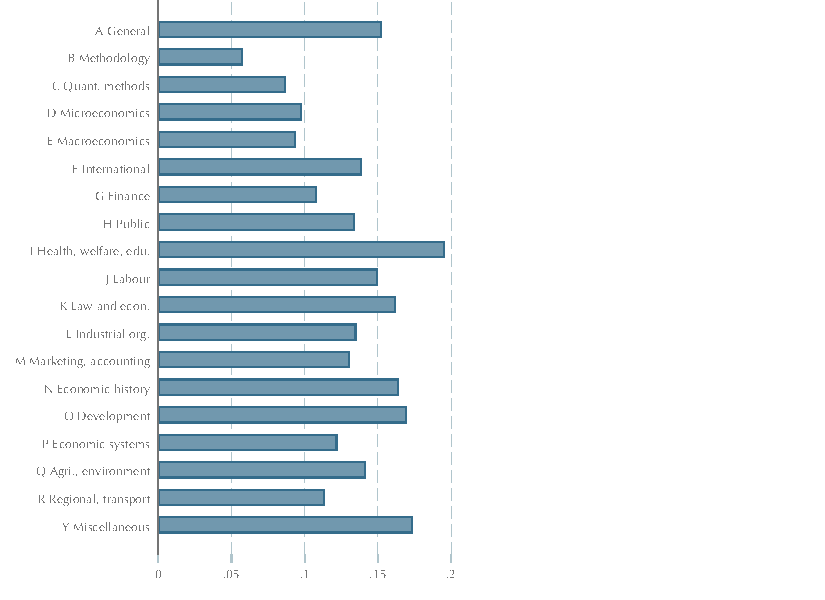
\includegraphics[trim=0cm 0cm 6cm 0cm, clip, width=\linewidth]{/Users/erinhengel/Dropbox/Readability/draft/pdf/jel.pdf}
	\end{minipage}
	\begin{minipage}{0.45\textwidth}
		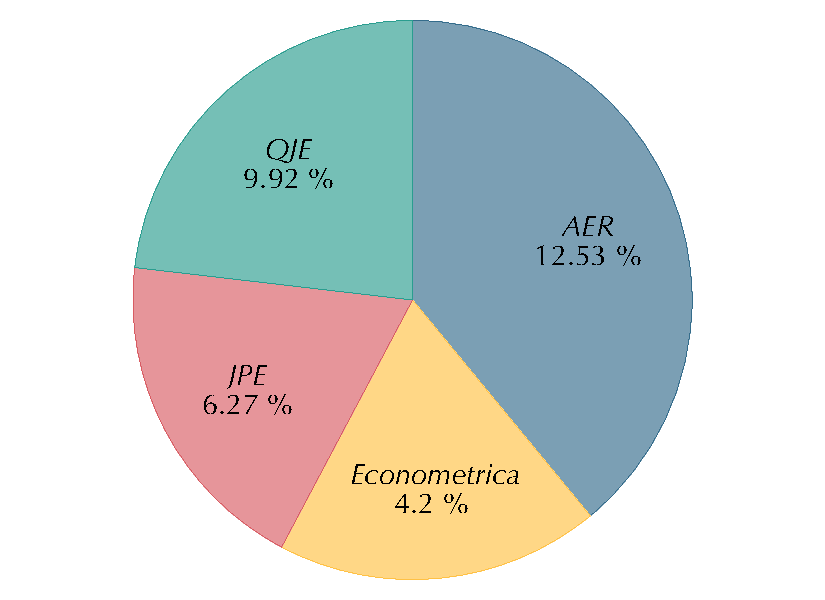
\includegraphics[width=0.95\linewidth]{/Users/erinhengel/Dropbox/Readability/draft/pdf/journal.pdf}
		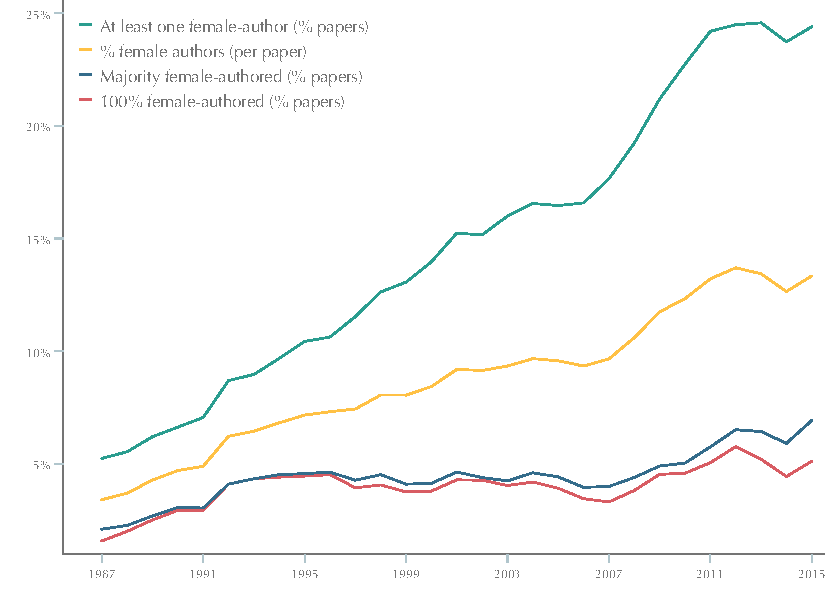
\includegraphics[width=0.95\linewidth]{/Users/erinhengel/Dropbox/Readability/draft/pdf/figure00.pdf}
	\end{minipage}
		\floatfoot{\tiny \textit{Notes}. First graph (upper left-hand corner) shows the percentage of all papers published in top economics journals that authored by more than 50 percent women; second graph (upper right-hand corner) is the percentage of all papers with at least one female author. Third graph (lower left-hand corner) shows the number of so-female-authored papers expressed as a percentage of all solo-authored papers. Final graph (lower right-hand corner) is the average ratio of female authors. See~\autoref{table1} for sample sizes broken down by journal and ten-year increments.}
	}
\end{figure}